\section{Method}
\label{sec:method}
\subsection{Forward model and prior}
\label{sec:forward}
Let $x \in \R^n$ be the unknown image and $\meas = \fwd x + \eta$ the measurement with $\eta \sim \mathcal{N}(0, \sigma^2 I)$. A pretrained score network $\score(x_t, t)$ approximates $\nabla \log p_t(x_t)$ along the noising process. Posterior sampling adds the likelihood gradient
\begin{equation}
  g_t = \nabla_{x_t} \norm{\meas - \fwd \xhat(x_t)}_2^2
  \label{eq:guidance}
\end{equation}
to the reverse update, where $\xhat(x_t)$ is Tweedie's estimate of the clean image~\cite{efron2011tweedie}.

\subsection{Score anchoring}
\label{sec:anchoring}
At each reverse step we compare the guidance gradient with the prior score and clip its contribution to a trust region:
\begin{equation}
  \anchor_t = g_t \cdot \min\!\left(1, \frac{\kap \norm{\score(x_t, t)}_2}{\norm{g_t}_2}\right).
  \label{eq:anchor}
\end{equation}
The anchor ratio $\kap$ is the only new hyperparameter. \Cref{eq:anchor} costs one norm per step and no extra evaluations of $\score$. When the guidance is small relative to the score the rule is the identity; when it is large the rule scales it down so that its norm never exceeds $\kap$ times that of the score.

\begin{figure}[t]
  \centering
  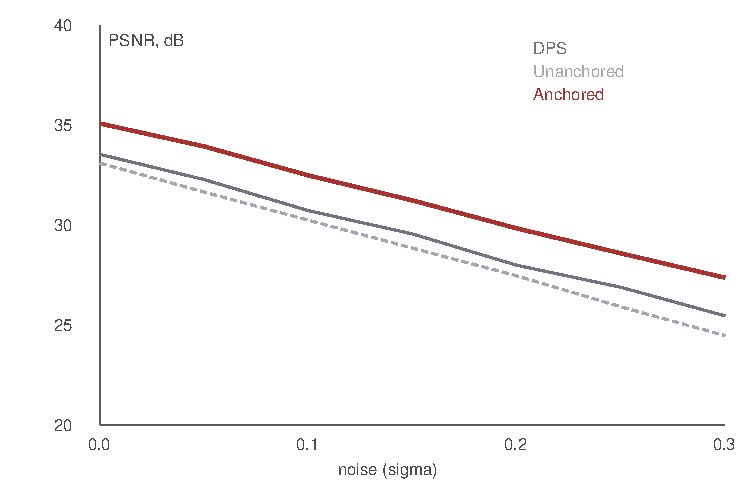
\includegraphics[width=\linewidth]{figures/anchor-schematic.pdf}
  \caption{The anchored update. The guidance gradient $g_t$ (red) is clipped to a ball of radius $\kap \norm{\score}$ around the current iterate before it is added to the prior score (blue). The direction of $g_t$ is unchanged.}
  \label{fig:schematic}
\end{figure}

\subsection{Samplers}
\label{sec:samplers}
Anchoring touches only $g_t$, so it drops into any sampler that exposes the guidance term. \Cref{alg:anchored} states the rule for a generic reverse step; \cref{app:samplers} spells it out for DDIM~\cite{song2021ddim}, the predictor--corrector sampler of~\cite{song2021sde} and the stochastic sampler of~\cite{karras2022edm}.

\begin{algorithm}[t]
\caption{One anchored reverse step}
\label{alg:anchored}
\begin{algorithmic}[1]
\Require $x_t$, $t$, measurement $\meas$, anchor ratio $\kap$
\State $s \gets \score(x_t, t)$
\State $g \gets \nabla_{x_t} \norm{\meas - \fwd \xhat(x_t)}_2^2$
\State $g \gets g \cdot \min(1, \kap \norm{s}_2 / \norm{g}_2)$
\State \Return $\textsc{ReverseStep}(x_t, s + g, t)$
\end{algorithmic}
\end{algorithm}

\subsection{Choosing the anchor ratio}
\label{sec:choosing-kappa}
We use $\kap = 1$ everywhere. \Cref{sec:ablation-kappa} shows that any value in $[0.5, 2]$ gives results within 0.2 dB of the reported numbers, so we do not tune $\kap$ per task.
